
\section{Experiment}

We evaluate the effectiveness of our MLP method with the Hopfield original network on MER(Message error) and BER(Bit error). We also do many experiments on different weight setting method of Hopfield network on different noise level. We do the experiments like Hopfield's original paper. The details of the datasets, the models and the training routines are summarized below.

\subsection{Datasets}

Our experiments are simulation. So the datasets are generated random. In our experiments, the Hopfield network's size are 30 and 100. The number of memory messages are 2,4,6 on 30 size, 10,15,20 on 100 size. For instance, we random generate 10 messages on 100 size. Every message is drown from a length of 100 $Ber(1/2)$ sequence. So message is a $100$ dimension binary vector, and every position choose from $\{-1, 1\}$ with probability $1/2$. Then for every position of every memory message, we generate 300 noise vectors by the following rule. For every position of memory message, we reverse its value, i.e 1 to -1, or -1 to 1, with probability of noise level. The noise levels we used are 0.05, 0.1, 0.2, 0.3.

There are two datasets. First, for every noise level, we generate memory messages. Then we generate the training set and testing set on this noise level. Second, on noise level 0.3, we generate memory messages, and generate training set. Then we according to these messages, generate testing set on noise level 0.1, 0.2, 0.3.

After this, we get a size of 3k training sets. Then we use the same method to generate the testing sets of which size is also 3k. In summary, on size 30, for message memory 2, we get 600 dataset. For message memory 4, we get 1.2k dataset. For message memory 6, we get 1.8k dataset. On size 100, for message memory 10, we get 3k dataset. For message memory 15, we get 4.5k dataset. For message memory 20, we get 6k dataset.

\subsection{Models and Implementation details}
\subsubsection{Hopfield method}

There are three Hopfield method. First is the Hopfield original paper. We call it HOP. Its idea of weight setting comes from Hebbian learning. Second is the pseudo-inverse method, called PSE. Third is the Storkey method, called STO. All these methods have a common property which don't need training step. The parameter weight of system is set only by the memory messages. So we just evaluate it on testing set.

\subsubsection{Machine learning method}

There is a new method different from the Hopfield method, called MPF. Its idea comes from minimum probability flow(MPF). It is a method similar to machine learning method. Cause we need to minimise a objective function to get the optimal weight. The difference is the objective function. In our method, we minimise the Euclid distance in training set. But the MPF minimise the energy between the message and its neighborhood. Our method is true from machine learning. We construct the training set according to our goals. So our methods can get better results on this task in theory. And the experiments also exhibit this result.

\subsubsection{Evaluation metric}

There are three metrics to evaluate the efficient between different methods. First, we call it MER, mean message's error. It requires that all the bit of message is the same with the target message. The second metric is BER, which means the bit error. The third metric is the most important metric, we call it Instability. Though the recovery is our objective, the memory messages are stable point.

\subsection{Results}

\subsubsection{Experiment I}

We do these experiments on 100 nodes. The memory messages are 10, 15 and 20. This experiment showed that our method MLP consistently superior to the antecedent weight setting method in all three metrics.

First in 10 memory messages. On noise level 0.05, 0.1, and 0.2, our MLP method is same efficiency with PSE and STO on metric MER, BER and Ins. On noise level 0.3, we can find the superiority of our method. Our MLP method is better than PSE, then STO, then MPF, and the last is HOP on MER and BER. About the Ins, the experiments show that MLP, PSE and STO all stable in all noise level. The worst result is HOP, but 0.04 is on 10 messages. So the wrong message is less than 1. Because we do the same experiment on 50 trial. This result is the mean of all these 50 trails. Maybe in some trials, there are two memory message is similar, so one of them is not stable.

%\begin{figure*}[!h]
%  \begin{minipage}{0.35\linewidth}
%    \centering
%    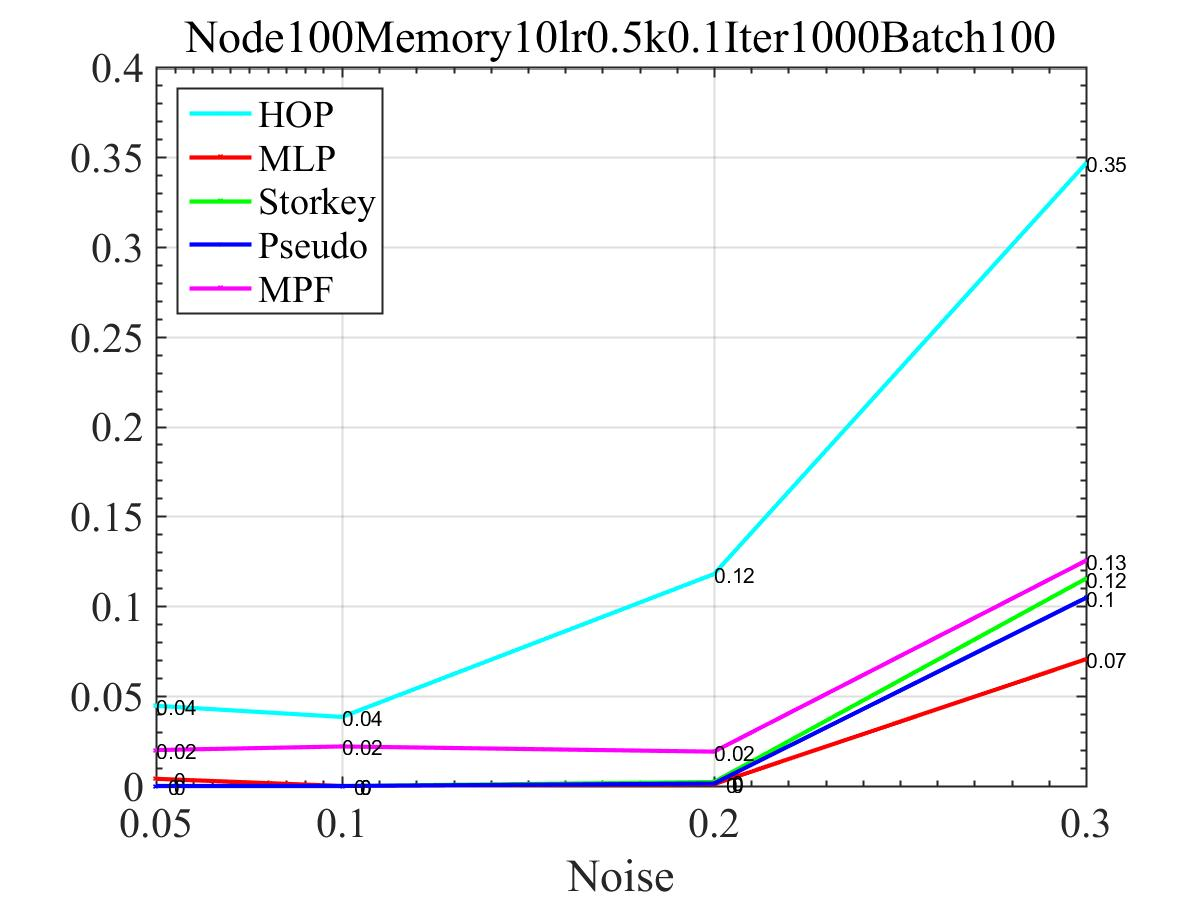
\includegraphics[width=0.8\textwidth]{Memory10MER.jpg}
%    \label{fig:figure1a}
%  \end{minipage}
%  \begin{minipage}{0.35\linewidth}
%    \centering
%    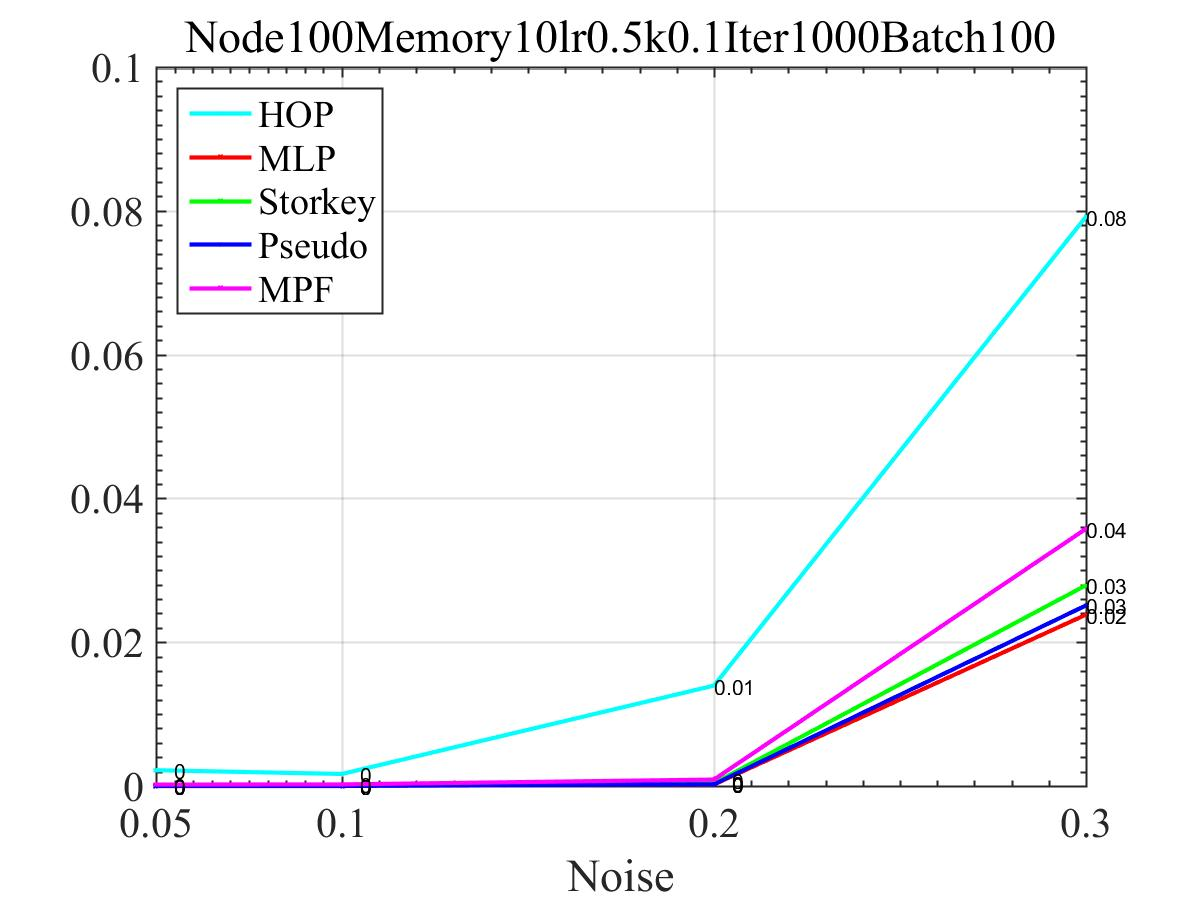
\includegraphics[width=0.8\textwidth]{Memory10BER.jpg}
%    \label{fig:figure1b}
%  \end{minipage}
%  \begin{minipage}{0.35\linewidth}
%    \centering
%    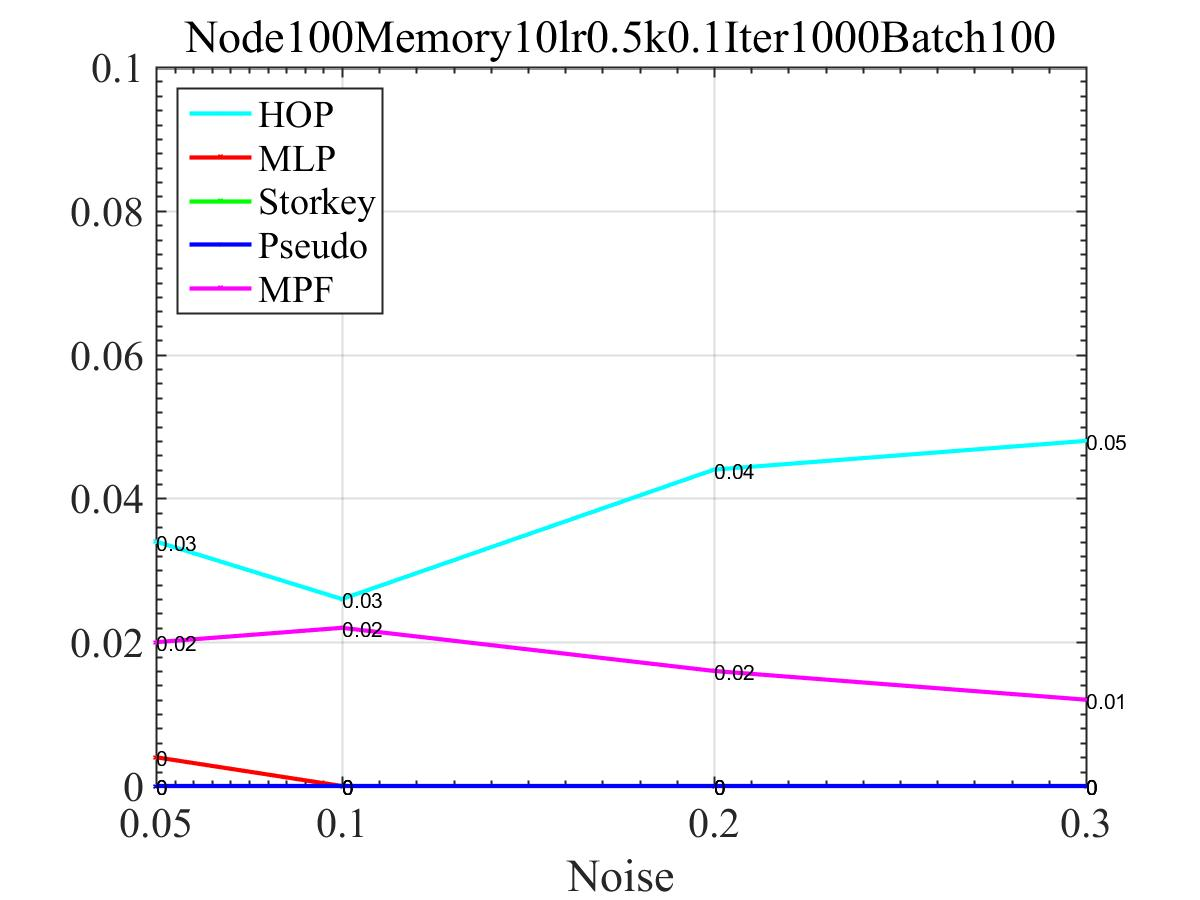
\includegraphics[width=0.8\textwidth]{Memory10Ins.jpg}
%    \label{fig:figure1c}
%  \end{minipage}
%  \caption{Memory10}
%\end{figure*}

\begin{figure*}[!h]
  \subfigure[MER]{
  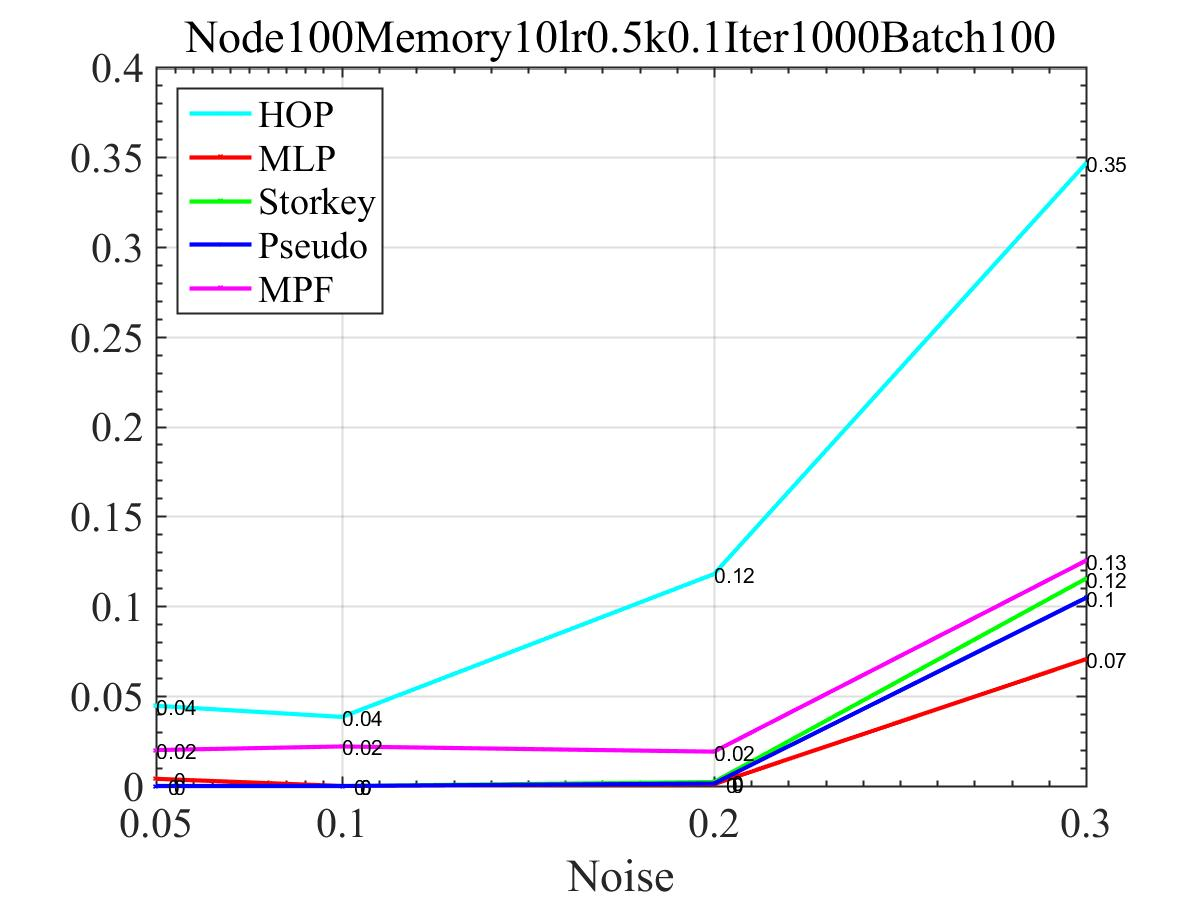
\includegraphics[width=0.35\textwidth]{Memory10MER.jpg}}
  \subfigure[BER]{
  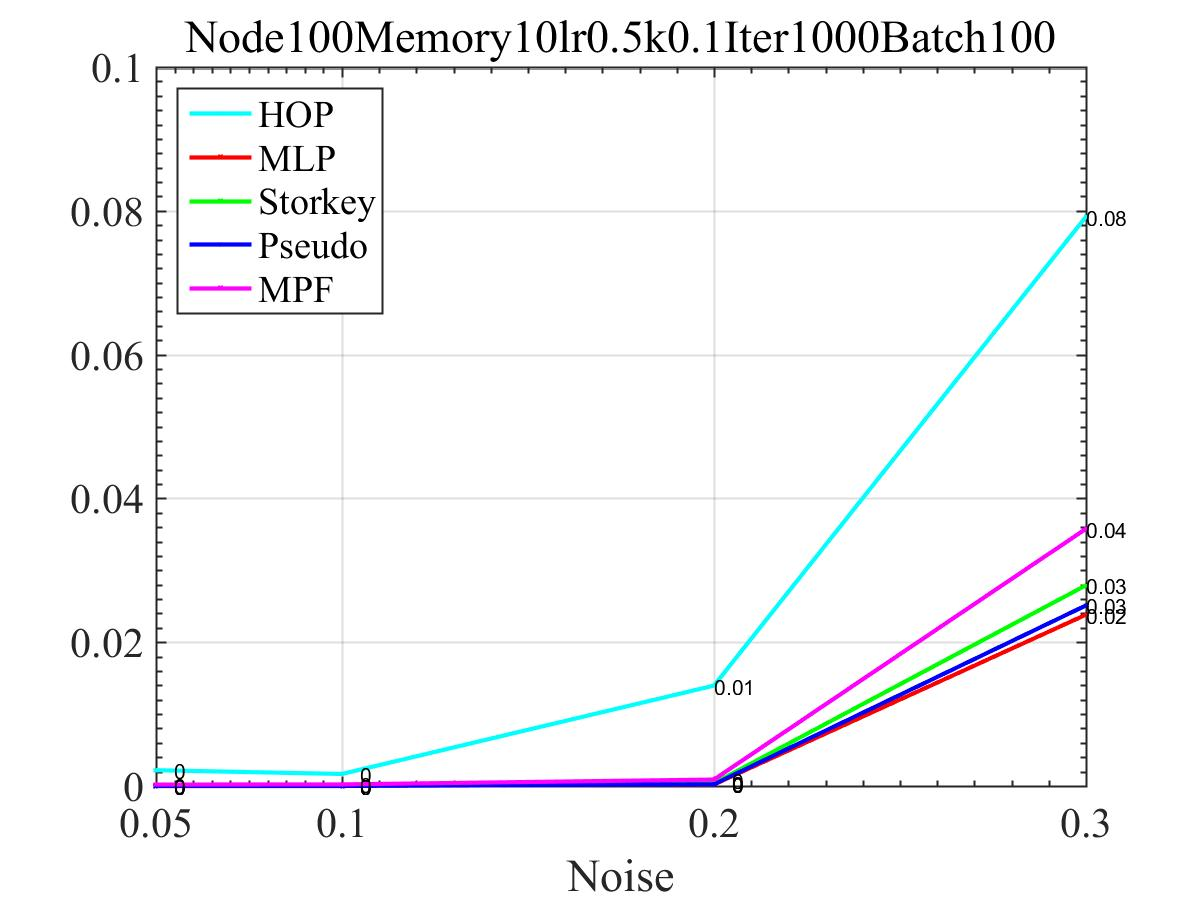
\includegraphics[width=0.35\textwidth]{Memory10BER.jpg}}
  \subfigure[Ins]{
  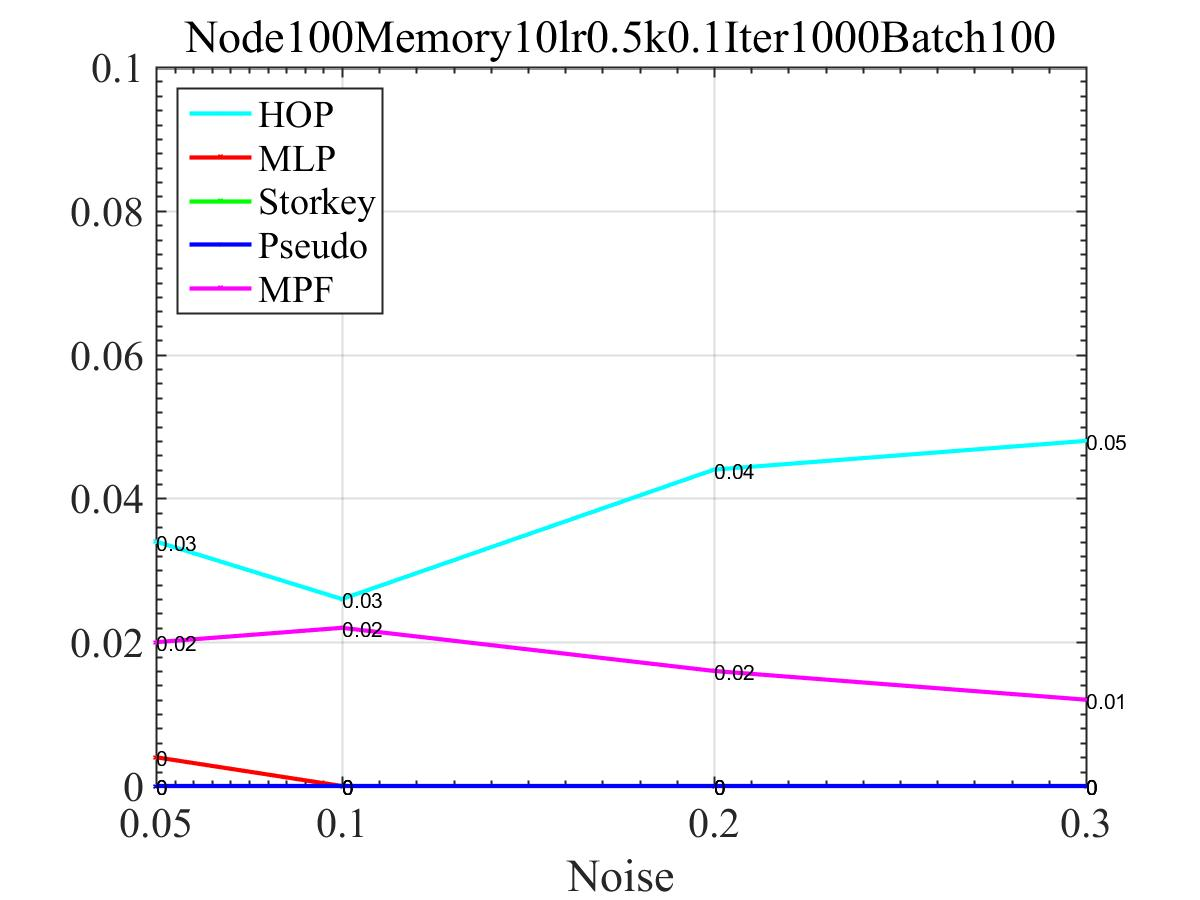
\includegraphics[width=0.35\textwidth]{Memory10Ins.jpg}}
  \caption{Memory10}
  \label{fig:fig1}
\end{figure*}


Second in 15 memory messages. Since the number of memory messages exceeds the capacity of Hopfield original network. In figure \ref{fig:fig2}, in all noise level, the error is about 3 memory messages of 15 memory messages. This accords with the theory of capacity of Hopfield network which the capacity is 0.14$N$. And on noise level 0.05, the MLP method have 0.03 error rate. This causes that MER also have 0.03 error rate.  But MPF, PSE, STO and our method MLP are almost stable on memory messages. So in figure \ref{fig:fig2} and \ref{fig:fig2}, on noise level 0.05, 0.1, and 0.2, the error rate is almost the same in all methods except HOP on metric MER and BER. The advantage of our method MLP is on noise level 0.3, both on metric MER and BER, our method MLP superior to MPF, then PSE, then STO, last is HOP.

\begin{figure*}[!h]
  \subfigure[MER]{
  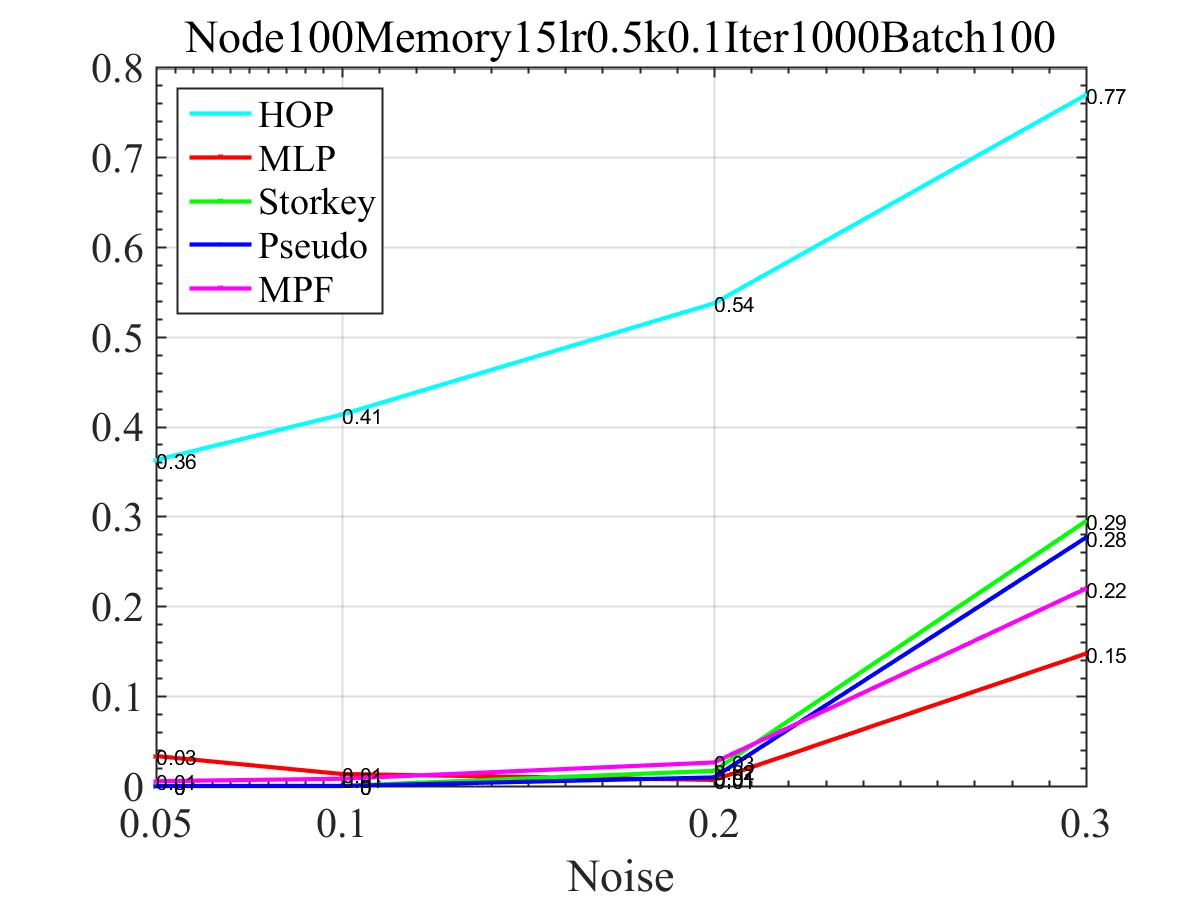
\includegraphics[width=0.35\textwidth]{Memory15MER.jpg}}
  \subfigure[BER]{
  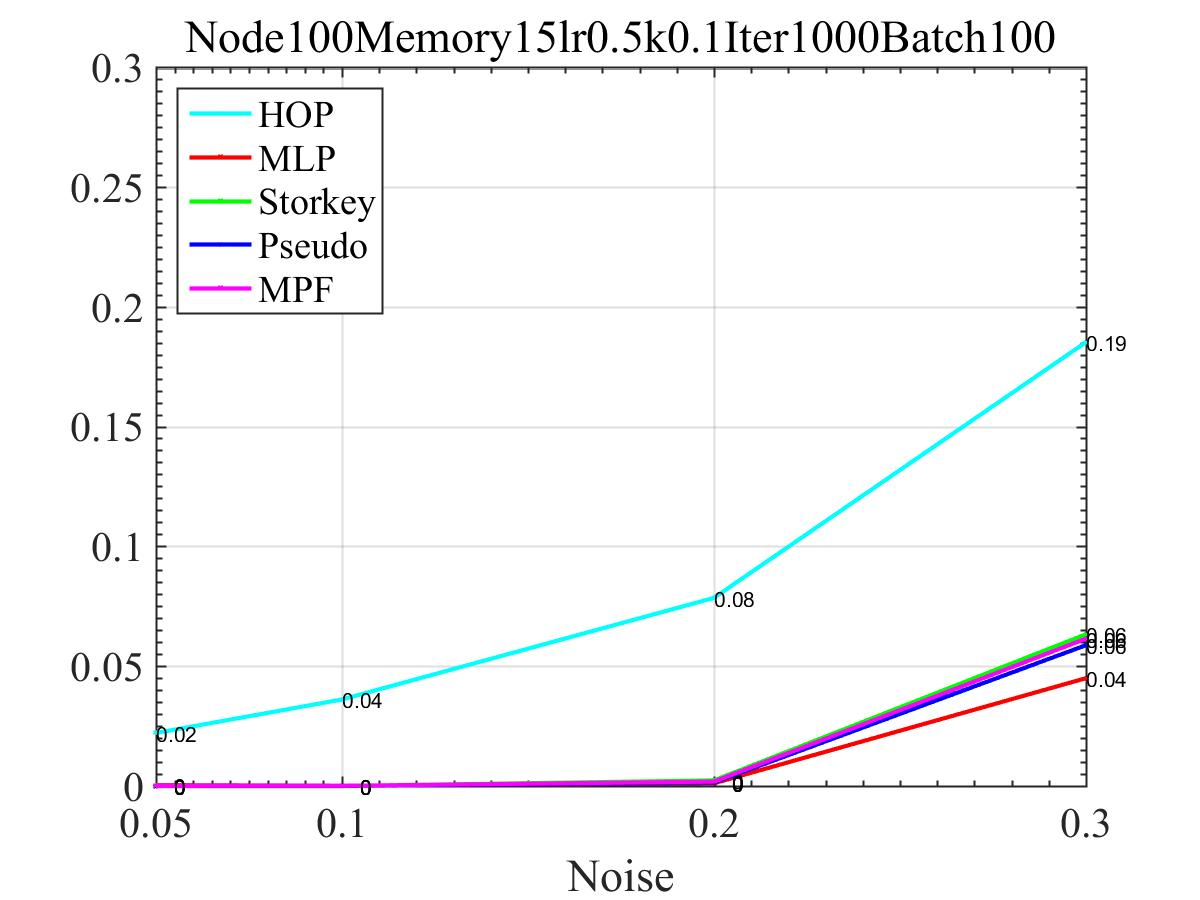
\includegraphics[width=0.35\textwidth]{Memory15BER.jpg}}
  \subfigure[Ins]{
  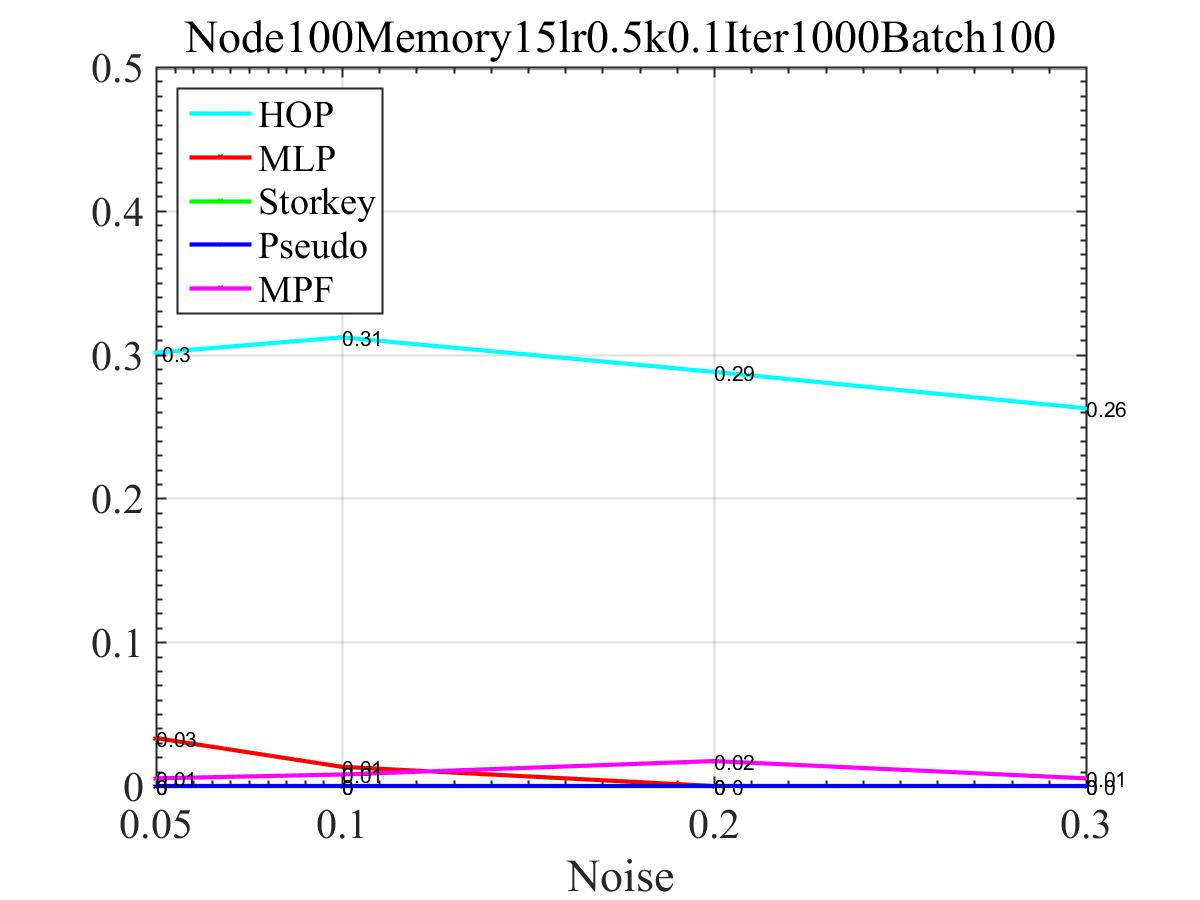
\includegraphics[width=0.35\textwidth]{Memory15Ins.jpg}}
  \caption{Memory15}
  \label{fig:fig2}
\end{figure*}
%
%\begin{figure}
%  \centering
%  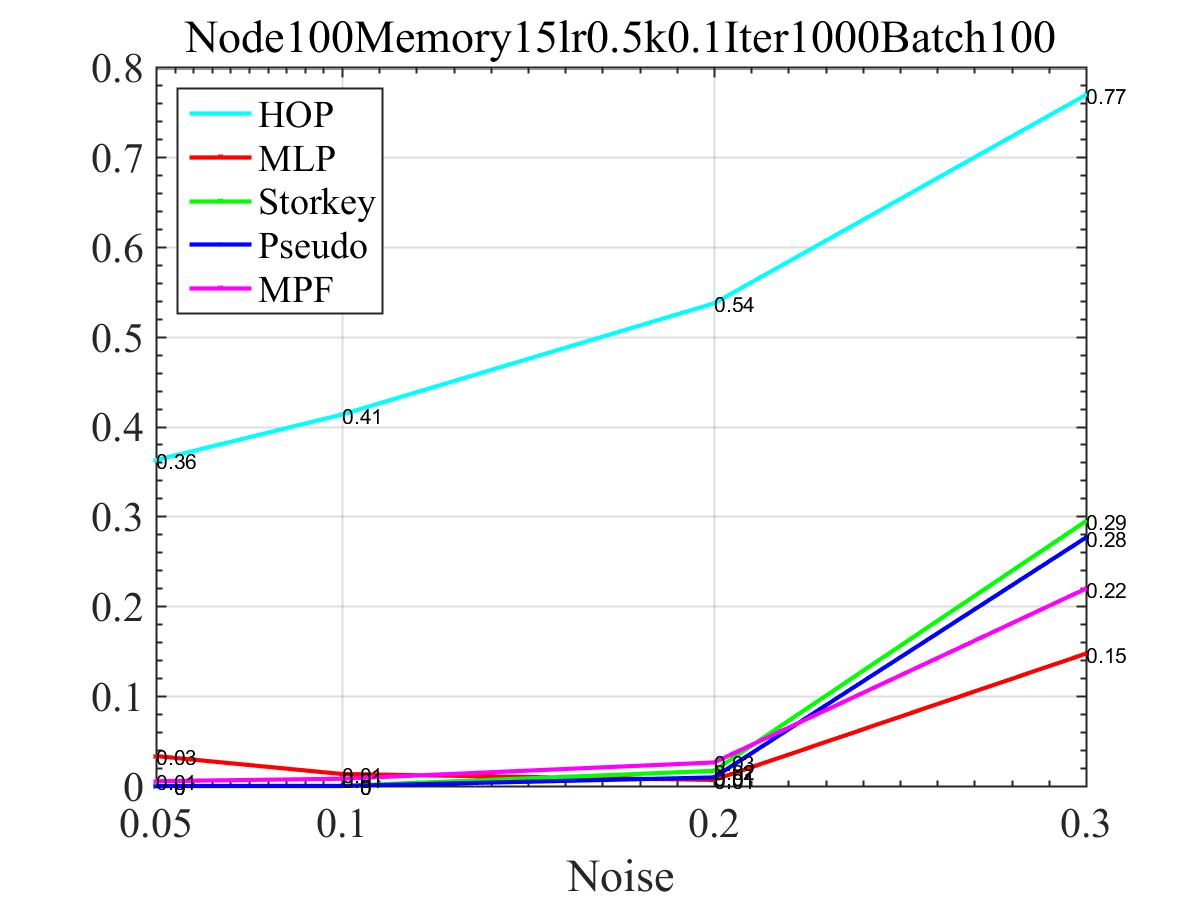
\includegraphics[width=2.2in]{Memory15MER.jpg}
%  \caption{Memory15MER}\label{fig:side:2a}
%\end{figure}
%\begin{figure}
%  \centering
%  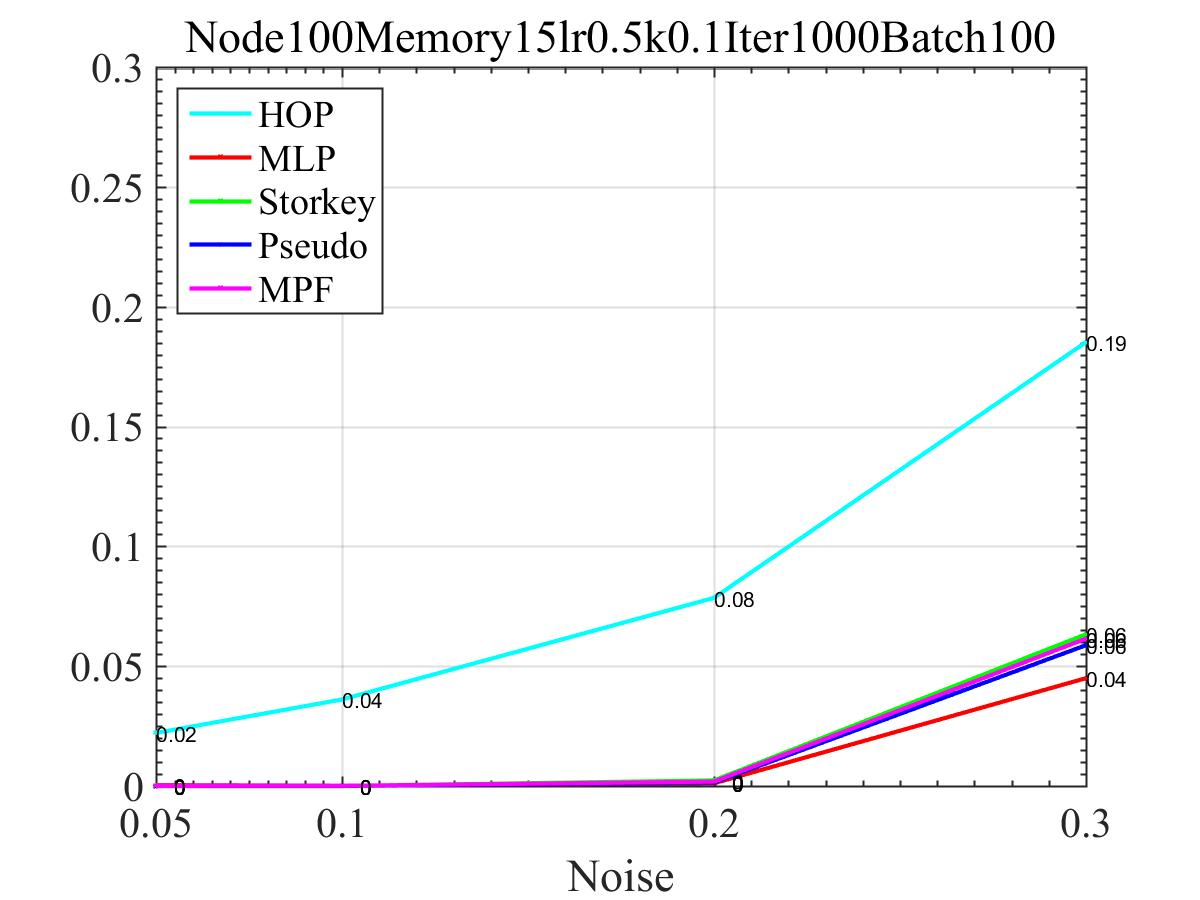
\includegraphics[width=2.2in]{Memory15BER.jpg}
%  \caption{Memory15BER}\label{fig:side:2b}
%\end{figure}
%\begin{figure}
%  \centering
%  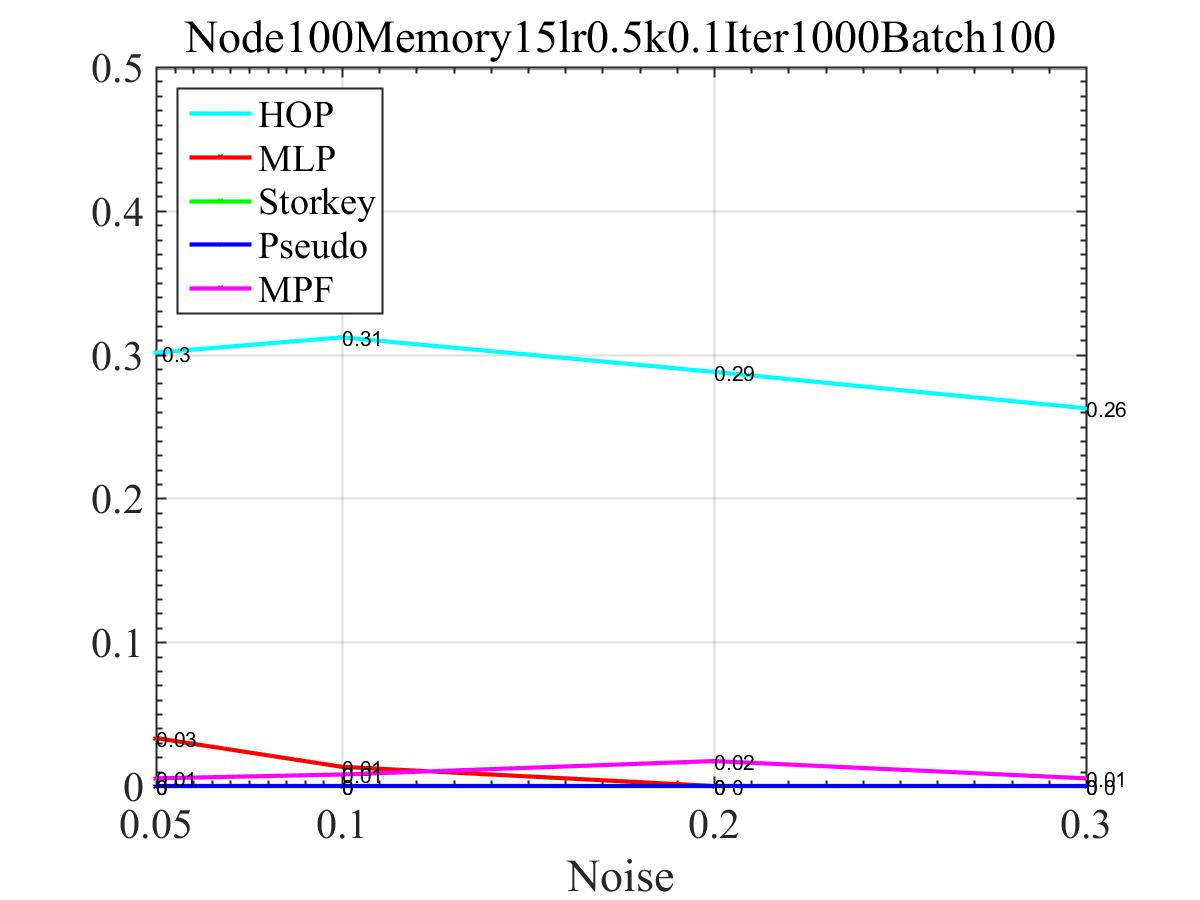
\includegraphics[width=2.2in]{Memory15Ins.jpg}
%  \caption{Memory15Ins}\label{fig:side:2c}
%\end{figure}

Third in 20 memory messages. Since the number of memory messages exceeds the capacity of Hopfield original network too more. In figure \ref{fig:fig3}, in all noise level, the error is about 12 memory messages of 20 memory messages. This also accords with the theory of capacity of Hopfield network which the capacity is 0.14$N$. And on noise level 0.05, the MLP method have 0.06 error rate. Besides on noise level 0.1, the MLP method have 0.03 error rate. This causes that MER also have 0.03 error rate.  But MPF, PSE, STO and our method MLP are almost stable on memory messages. So in figure \ref{fig:fig3} and \ref{fig:fig3}, on noise level 0.05, 0.1, and 0.2, the error rate is almost the same in all methods except HOP on metric MER and BER. The superiority of our method MLP is on noise level 0.3, both on metric MER and BER, our method MLP superior to MPF, then PSE, then STO, last is HOP.

\begin{figure*}[!h]
  \subfigure[MER]{
  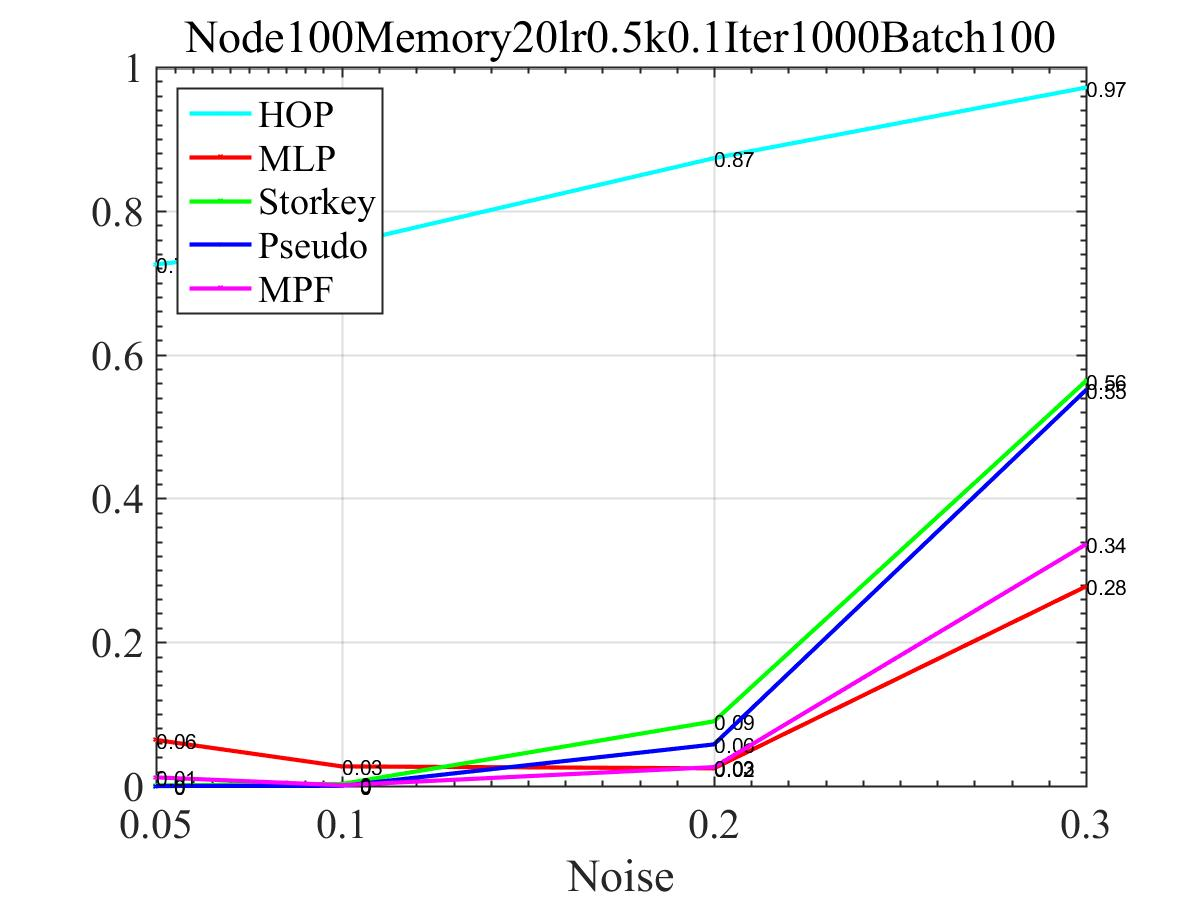
\includegraphics[width=0.35\textwidth]{Memory20MER.jpg}}
  \subfigure[BER]{
  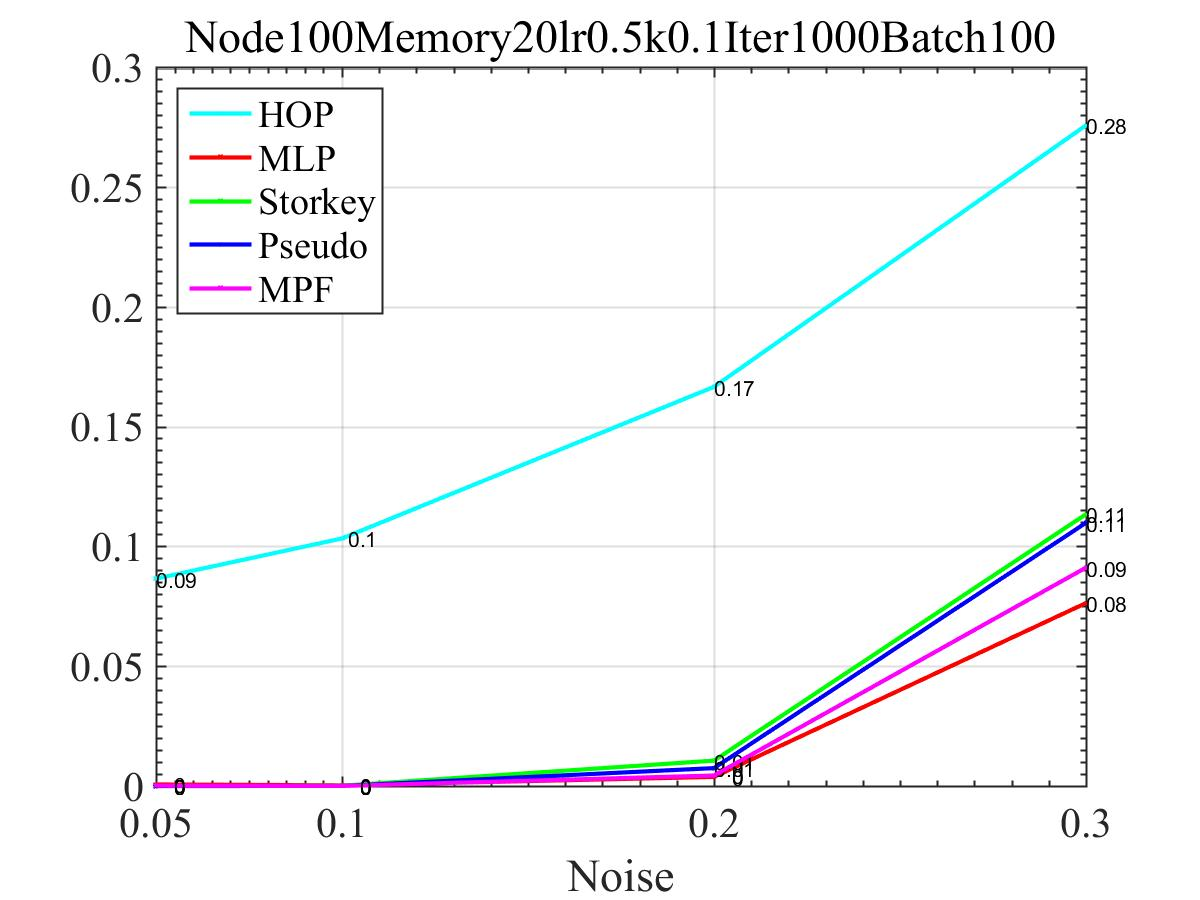
\includegraphics[width=0.35\textwidth]{Memory20BER.jpg}}
  \subfigure[Ins]{
  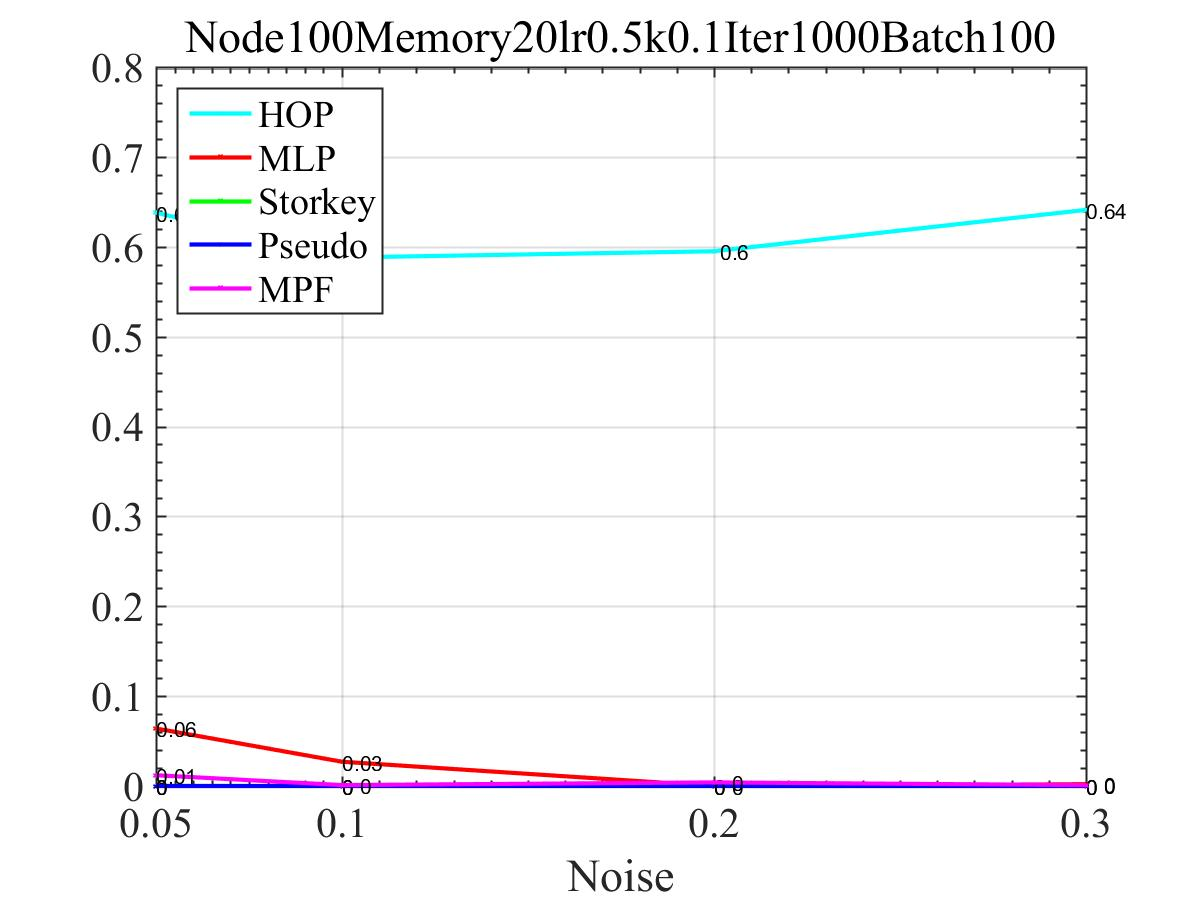
\includegraphics[width=0.35\textwidth]{Memory20Ins.jpg}}
  \caption{Memory20}
  \label{fig:fig3}
\end{figure*}

%\begin{figure}
%  \centering
%  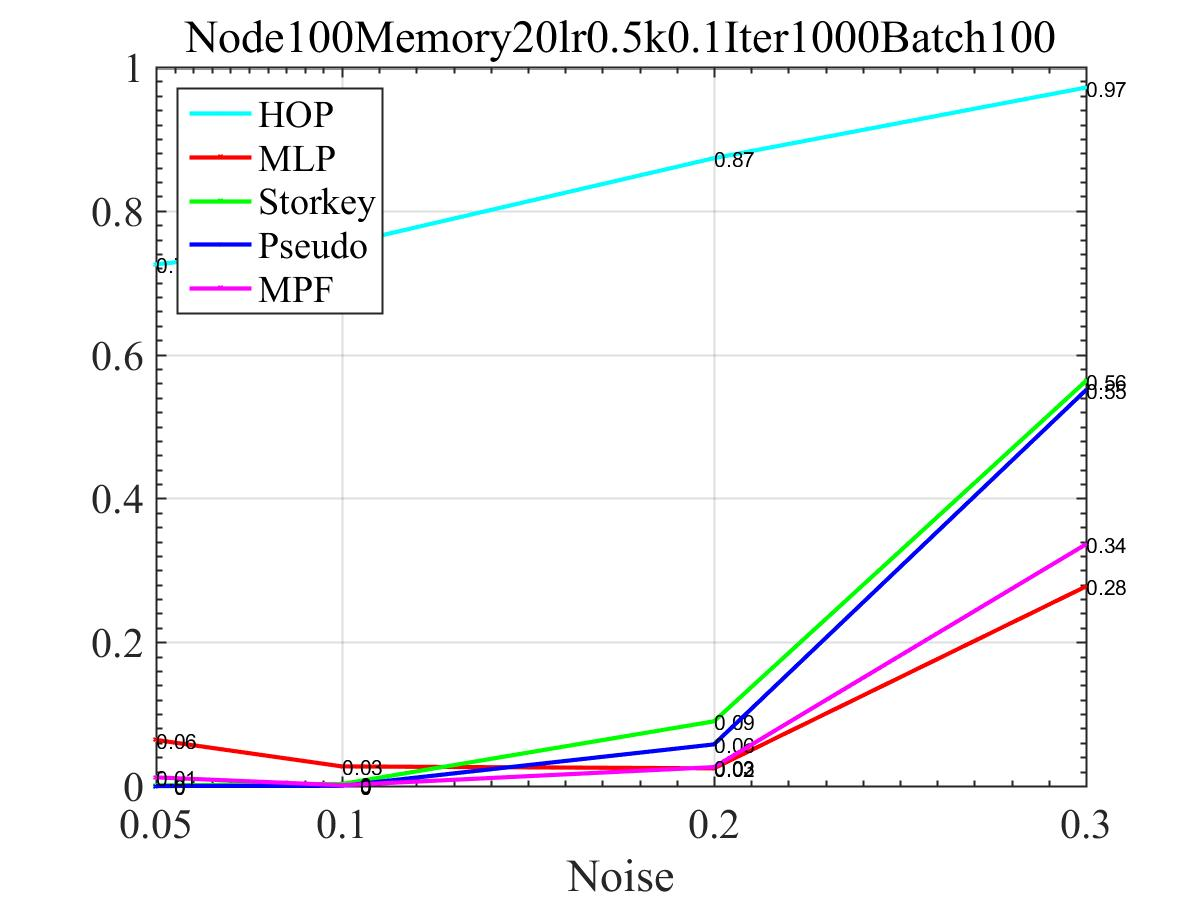
\includegraphics[width=2.2in]{Memory20MER.jpg}
%  \caption{Memory20MER}\label{fig:side:3a}
%\end{figure}
%\begin{figure}
%  \centering
%  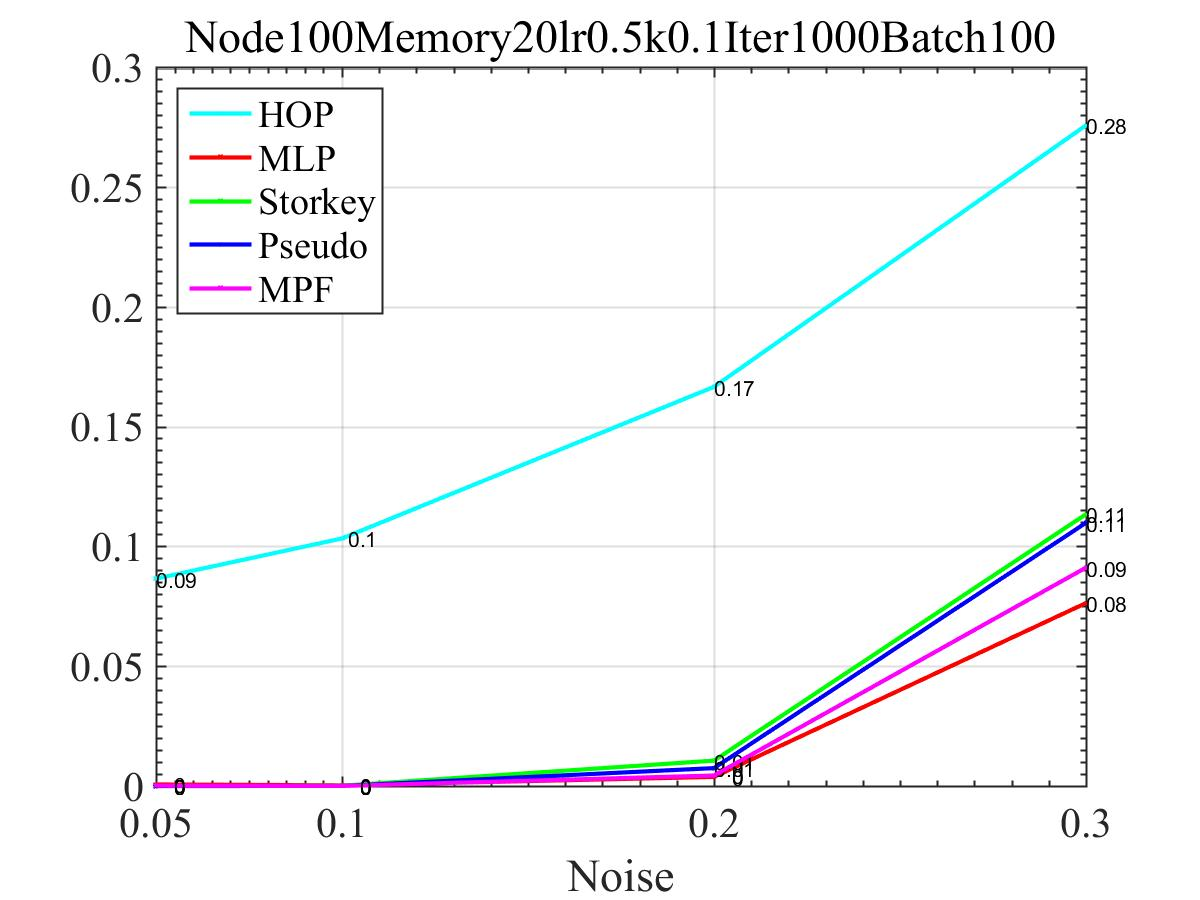
\includegraphics[width=0.48\textwidth]{Memory20BER.jpg}
%  \caption{Memory20BER}\label{fig:side:3b}
%\end{figure}
%\begin{figure}
%  \centering
%  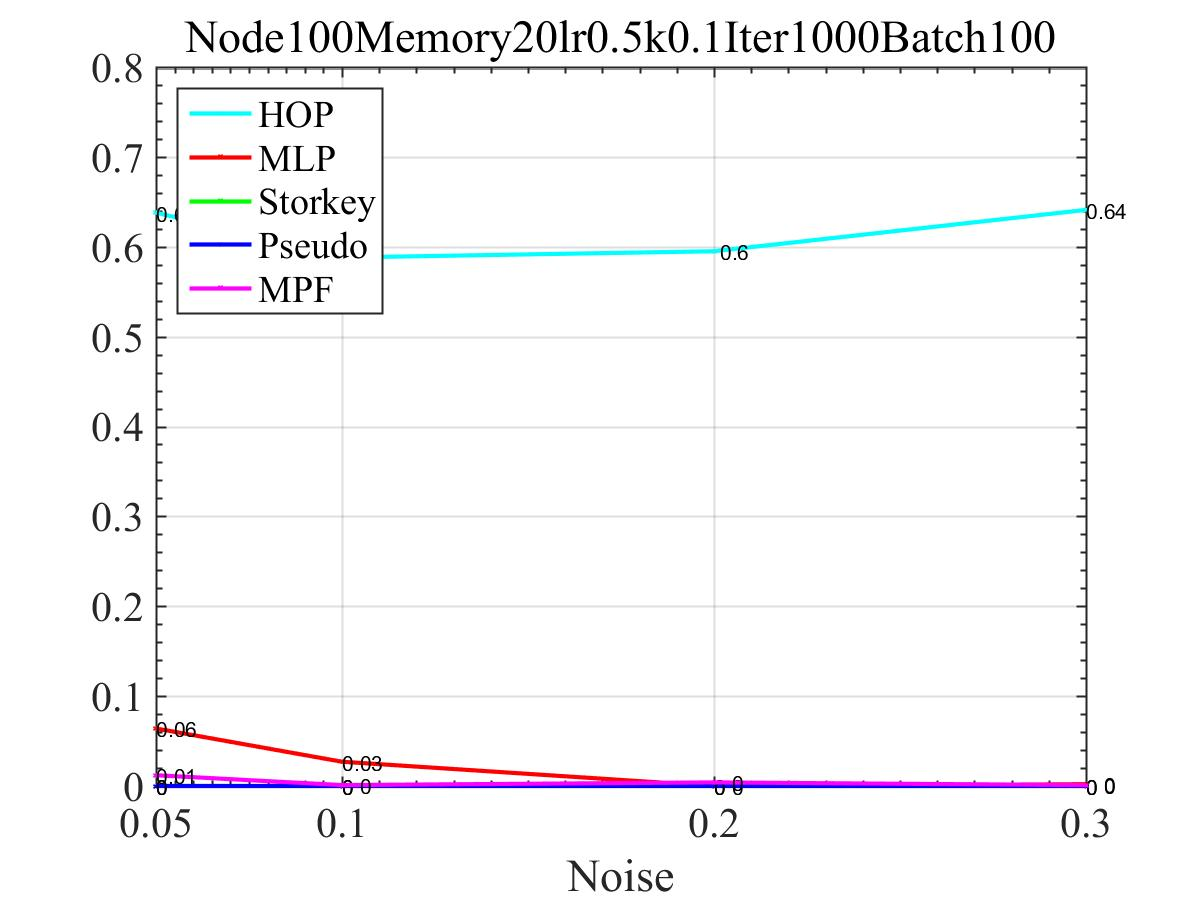
\includegraphics[width=0.48\textwidth]{Memory20Ins.jpg}
%  \caption{Memory20Ins}\label{fig:side:3c}
%\end{figure}

In summary, the weight comes from our method MLP, can make Hopfield network recover better, particularly on high noise level. When we train our Hopfield network on low noise level, maybe we cannot get the exact solution. So we try another experiment, we just train on high noise level, i.e 0.3, we test the Hopfield network on 0.1, 0.2, and 0.3. The following is the results.

\subsubsection{Experiments II} 

In these experiment II, we train our Hopfield network on high noise level, i.e 0.3 noise level. Then we do testing work on all the noise level 0.1, 0.2 and 0.3. The following figure is the results.

When there are 10 memory messages, we find that our method MLP is superior to HOP in all metric, MER, BER and Ins.
%\begin{figure}
%  \centering
%  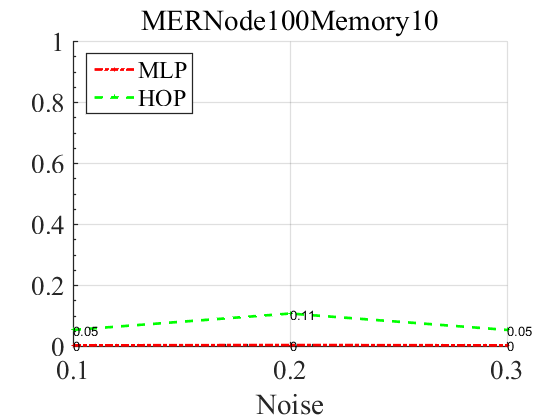
\includegraphics[width=0.48\textwidth]{E2Node100Memory10MER.png}
%  \caption{Memory10MER}\label{fig:side:4a}
%\end{figure}
%\begin{figure}
%  \centering
%  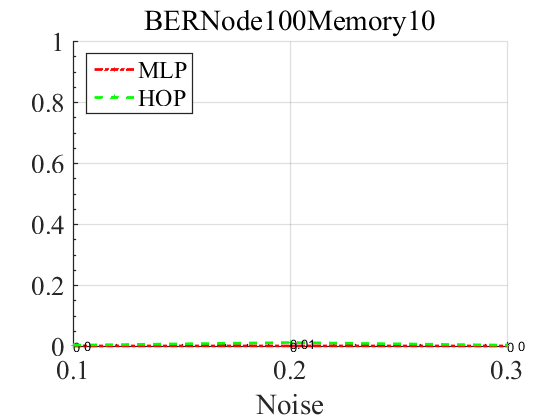
\includegraphics[width=0.48\textwidth]{E2Node100Memory10BER.png}
%  \caption{Memory10BER}\label{fig:side:4b}
%\end{figure}
%\begin{figure}
%  \centering
%  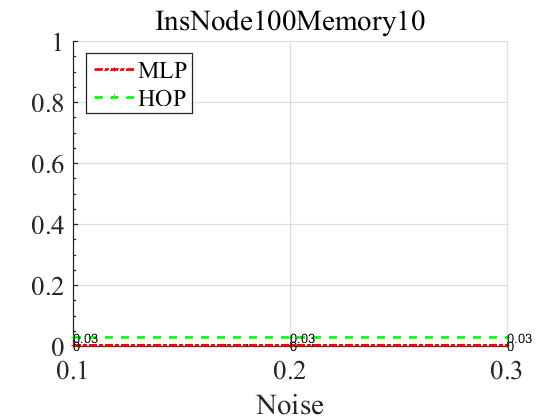
\includegraphics[width=0.48\textwidth]{E2Node100Memory10Ins.png}
%  \caption{Memory10Ins}\label{fig:side:4c}
%\end{figure}

When there are 15 memory messages, we find that our method MLP is superior to HOP in all metric, MER, BER and Ins.

%\begin{figure}
%  \centering
%  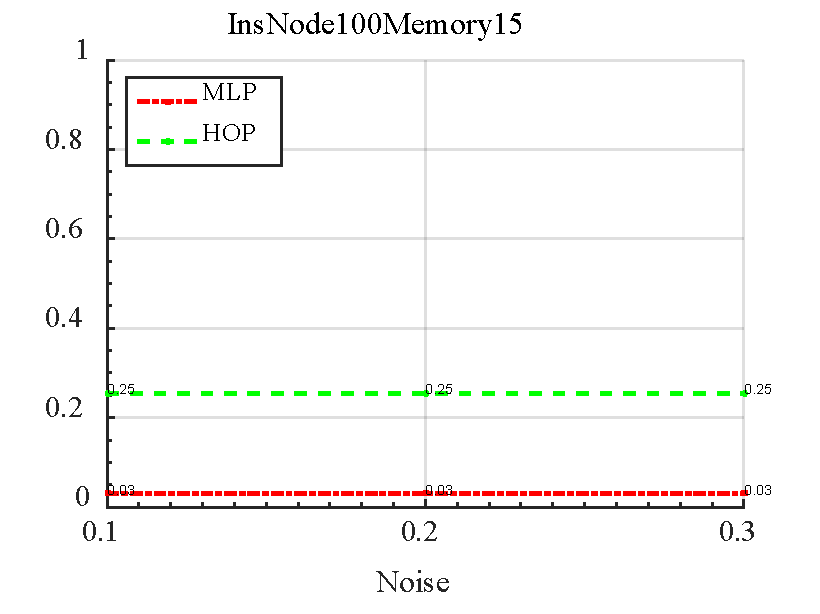
\includegraphics[width=0.48\textwidth]{Memory15Ins.pdf}
%  \caption{Memory15MER}\label{fig:side:5a}
%\end{figure}
%\begin{figure}
%  \centering
%  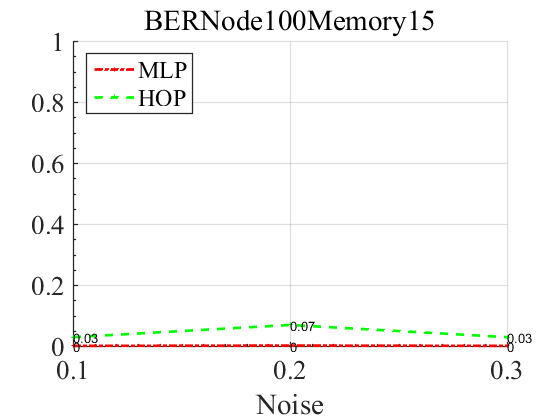
\includegraphics[width=0.48\textwidth]{E2Node100Memory15BER.png}
%  \caption{Memory15BER}\label{fig:side:5b}
%\end{figure}
%\begin{figure}
%  \centering
%  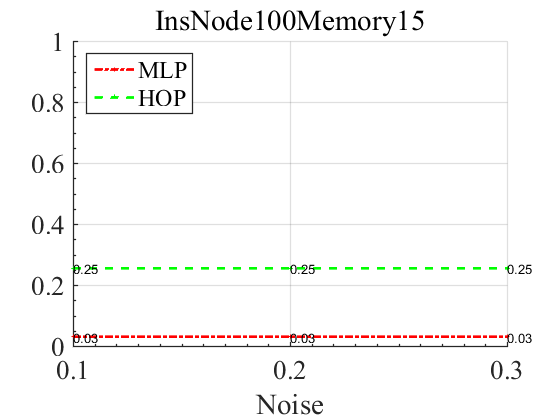
\includegraphics[width=0.48\textwidth]{E2Node100Memory15Ins.png}
%  \caption{Memory15Ins}\label{fig:side:5c}
%\end{figure}

When there are 20 memory messages, we find that our method MLP is superior to HOP in all metric, MER, BER and Ins.

%\begin{figure}
%  \centering
%  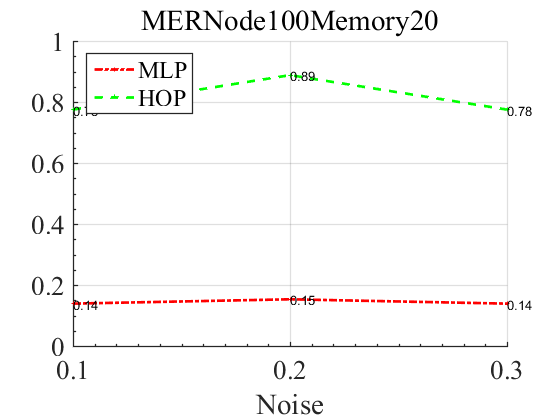
\includegraphics[width=0.48\textwidth]{E2Node100Memory20MER.png}
%  \caption{Memory20MER}\label{fig:side:6a}
%\end{figure}
%\begin{figure}
%  \centering
%  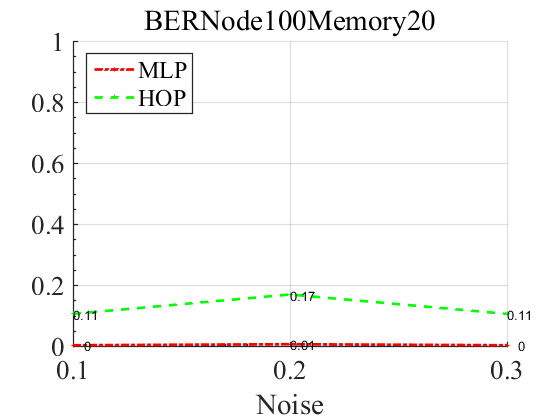
\includegraphics[width=0.48\textwidth]{E2Node100Memory20BER.png}
%  \caption{Memory20BER}\label{fig:side:6b}
%\end{figure}
%\begin{figure}
%  \centering
%  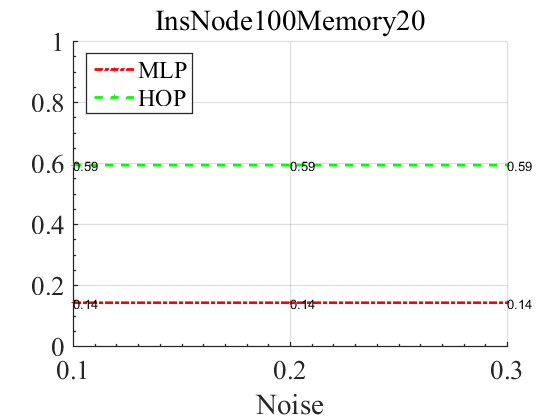
\includegraphics[width=0.48\textwidth]{E2Node100Memory20Ins.png}
%  \caption{Memory20Ins}\label{fig:side:6c}
%\end{figure}

In summary, in all three condition, our method MLP is superior to HOP 